\documentclass[11pt]{article}

% packages
\usepackage{enumerate}
\usepackage{fancyhdr}
\usepackage{extramarks}
\usepackage{amsmath}
\usepackage{amsthm}
\usepackage{amssymb}
%\usepackage{amsfonts}
\usepackage{tikz}
\usepackage[plain]{algorithm}
\usepackage{algpseudocode}
\usepackage{lastpage}
\usepackage{units}
\usepackage[margin=0.75in]{geometry}
\usepackage{pgfplots}
\pgfplotsset{compat=1.16}
\usepackage{sectsty}
\usepackage{hyperref}
\usepackage{multicol}
\usepackage{mathtools}
\usepackage{tikz}
\usetikzlibrary{matrix}
\usepackage{listings}
\usepackage[plain]{algorithm}
\usepackage{algpseudocode}
\usepackage{mdframed}

\definecolor{sblue}{HTML}{5292c0}
\definecolor{sgreen}{HTML}{93c47d}
\definecolor{sorange}{HTML}{e69138}
\definecolor{codeblue}{rgb}{0.29296875, 0.51953125, 0.68359375}
\definecolor{codegreen}{rgb}{0.47265625, 0.62890625, 0.40234375}
\definecolor{codegray}{rgb}{0.95703125, 0.95703125, 0.95703125}
\definecolor{codecrimson}{rgb}{0.87109375,0.3984375,0.3984375}

\lstset{frame=tb,
  backgroundcolor=\color{codegray},
  aboveskip=3mm,
  belowskip=3mm,
  showstringspaces=false,
  columns=flexible,
  basicstyle={\small\ttfamily},
  numbers=left,
  numberstyle=\tiny\color{gray},
  keywordstyle=\color{codeblue},
  commentstyle=\color{codegreen},
  stringstyle=\color{codecrimson},
  breaklines=true,
  breakatwhitespace=true,
  tabsize=4,
  frame=tlbr,framesep=4pt,framerule=0pt,
  literate={`}{\`}1,
}

% colors
\definecolor{sblue}{HTML}{5292c0}
\definecolor{sgreen}{HTML}{93c47d}
\definecolor{sorange}{HTML}{e69138}

% sectioning magic
\counterwithin*{equation}{section}
%\numberwithin{equation}{section}

% fonts
\usepackage{fontspec}
\newfontfamily\headerfontlt{ITC Franklin Gothic Std Book}
\newfontfamily\headerfont{ITC Franklin Gothic Std Demi}
\usepackage[urw-garamond]{mathdesign}
\usepackage{garamondx}
\usepackage[italic]{mathastext}

\newcommand{\printsection}[1]{\normalfont\headerfontlt{{{#1}}}}
\newcommand{\printsubsection}[1]{\normalfont\headerfontlt\textcolor{darkgray}{{#1}}}
\newcommand{\printsubsubsection}[1]{\normalfont\headerfontlt{{#1}}}
\allsectionsfont{\printsection}
\subsectionfont{\printsection}
\subsectionfont{\printsubsection}
\subsubsectionfont{\printsubsubsection}


\renewcommand{\headrulewidth}{0.1pt}
\renewcommand{\headrule}{\hbox to\headwidth{\color{gray}\leaders\hrule height \headrulewidth\hfill}}
\renewcommand{\footrulewidth}{0.0pt}

\newcommand{\op}[1]{\textrm{\small\printsubsection{\MakeUppercase{#1}}}\,}
\newcommand{\opns}[1]{\textrm{\small\printsubsection{\MakeUppercase{#1}}}}
\newcommand{\Partial}[1]{\partial\hspace{-0.2ex}{#1}}
\newcommand{\D}[1]{\mathrm{d}#1}
\newcommand{\E}[1]{\mathbb{E}{\left[\,#1\,\right]}}
\newcommand{\var}[1]{\mathrm{var}\left( #1 \right)}
\newcommand{\cov}[1]{\mathrm{cov}\left( #1 \right)}
\newcommand{\pr}[1]{\mathrm{Pr}\left( #1 \right)}
\newcommand{\given}{\,|\,}
\renewcommand{\det}{\mathrm{det\,}}
\renewcommand{\det}[1]{\op{det}\left(#1\right)}
\renewcommand{\ker}{\mathrm{Ker\,}}
\newcommand{\trace}[1]{\op{trace}\left(#1\right)}
\newcommand{\nul}[1]{\op{nul}\left(#1\right)}
\newcommand{\col}[1]{\op{col}\left(#1\right)}
\newcommand{\row}[1]{\op{row}\left(#1\right)}
\newcommand{\rank}[1]{\op{rank}\left(#1\right)}
\renewcommand{\dim}[1]{\op{dim}\left(#1\right)}
\newcommand{\im}{\op{Im\,}}
\newcommand{\reals}{\mathbb{R}}
\newcommand{\complex}{\mathbb{C}}
\renewcommand{\vec}[1]{\mathbf{#1}}
\newcommand*{\matr}[1]{\mathbfit{#1}}
\newcommand*{\tran}{^{\mkern-1.5mu\mathsf{T}}}
\newcommand*{\conj}[1]{\overline{#1}}
\newcommand*{\hermconj}{^{\mathsf{H}}}
\newcommand*{\inv}{^{-1}}

\setlength\parindent{0pt}
\pagecolor{gray!1}


% header/footer
\topmargin=-0.65in
\pagestyle{fancy}\fancyhf{} 
\lhead{\headerfontlt{\textcolor{darkgray}{Satej Soman \textcolor{gray}{$\big/$} CAPP30254, Spring 19 \textcolor{gray}{$\big/$}} Homework 1}}
\rhead{\headerfontlt{\textcolor{gray}{$\big[$} \thepage\ \textcolor{gray}{$\big/$} \pageref{LastPage} \textcolor{gray}{$\big]$}}}

\begin{document}
\begin{titlepage}
\raggedleft\huge\headerfontlt{
\textcolor{darkgray}{Satej Soman\\
CAPP30254: Machine Learning for Public Policy\\
Spring 2019}}

\vspace{240pt}
\Huge\headerfontlt{\textcolor{darkgray}{HW 1\\DIAGNOSTIC ASSIGNMENT}}

\end{titlepage}
\section*{Notes}
\begin{itemize}
\item Representative code snippets are interspersed with analysis and explanations below; all code is available on GitHub: \url{https://github.com/satejsoman/capp30254/tree/master/hw1/code}.
\item Sources for data and techniques are cited at the end of this report.
\end{itemize}

\section{Data Acquisition \& Analysis}
\subsection{Chicago Open Data Portal}
Chicago crime data is available, filtered by year, from the Chicago Data Portal (\url{https://data.cityofchicago.org/browse?category=Public\%20Safety}). We can download this data and load it into a Pandas \texttt{DataFrame}:

\begin{lstlisting}[language=Python,numbers=none]
from pathlib import Path

import pandas as pd
import requests

# download crime data if we don't have it locally
base_url = "https://data.cityofchicago.org/api/views/{}/rows.csv?accessType=DOWNLOAD"
crime_resources = { 
    2017: (Path("./crime_data_2017.csv"), "3i3m-jwuy"),
    2018: (Path("./crime_data_2018.csv"), "d62x-nvdr"),
}

for (year, (path, identifier)) in crime_resources.items():
    if not path.exists():
        url = base_url.format(identifier)
        print("{} data not found locally, downloading from {}".format(year, url))
        response = requests.get(url)
        with path.open("wb") as f:
            f.write(response.content)

crime_stats = pd.concat([
    pd.read_csv(crime_resources[2017][0]), 
    pd.read_csv(crime_resources[2018][0])
])
\end{lstlisting}


\subsection{Summary Statistics for Crime Report Data, 2017-2018}

\begin{table}[H]
\centering \renewcommand{\arraystretch}{1.2}
\begin{tabular}{lrrr}
\multicolumn{1}{l|}{year} &    \opns{2017} &    \opns{2018} &     \opns{AVG} \\\hline
\multicolumn{1}{l|}{number of reported crimes} &  268094 &  266246 &  267170 \\
\\ \\
%\end{tabular}
%\end{table}
%\begin{table}[H]
%\centering \renewcommand{\arraystretch}{1.2}
%\begin{tabular}{l|rrr}
\multicolumn{1}{l|}{year} &       \opns{2017} &  \opns{2018} &  \opns{OVERALL} \\\hline
\multicolumn{1}{l|}{crimes involving an arrest}   &  19.53\% &  19.75\% &  19.64\% \\
\multicolumn{1}{l|}{crimes considered domestic}   &  15.90\% &  16.39\% &  16.14\% 
\end{tabular}
\end{table}


{\centering
\hspace{-1in}% This file was created by matplotlib2tikz v0.7.3.
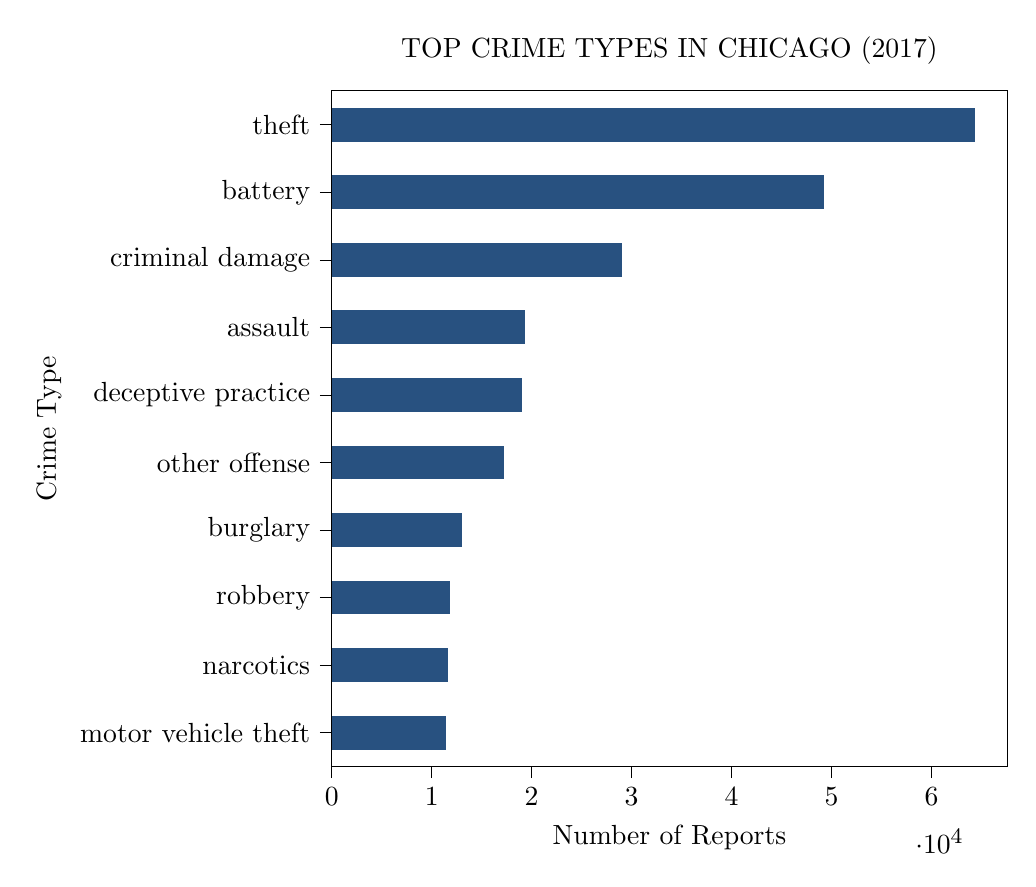
\begin{tikzpicture}

\definecolor{color0}{rgb}{0.156862745098039,0.317647058823529,0.501960784313725}

\begin{axis}[
height=4in,
tick align=outside,
tick pos=left,
title={\printsection{\MakeUppercase{Top Crime Types in Chicago (2017)}}},
width=4in,
x grid style={white!69.01960784313725!black},
xlabel={Number of Reports},
xmin=0, xmax=67562.25,
xtick style={color=black},
y grid style={white!69.01960784313725!black},
ylabel={Crime Type},
ymin=-0.5, ymax=9.5,
ytick style={color=black},
ytick={0,1,2,3,4,5,6,7,8,9},
yticklabels={motor vehicle theft,narcotics,robbery,burglary,other offense,deceptive practice,assault,criminal damage,battery,theft}
]
\draw[fill=color0,draw opacity=0] (axis cs:0,-0.25) rectangle (axis cs:11406,0.25);
\draw[fill=color0,draw opacity=0] (axis cs:0,0.75) rectangle (axis cs:11658,1.25);
\draw[fill=color0,draw opacity=0] (axis cs:0,1.75) rectangle (axis cs:11877,2.25);
\draw[fill=color0,draw opacity=0] (axis cs:0,2.75) rectangle (axis cs:13001,3.25);
\draw[fill=color0,draw opacity=0] (axis cs:0,3.75) rectangle (axis cs:17227,4.25);
\draw[fill=color0,draw opacity=0] (axis cs:0,4.75) rectangle (axis cs:19025,5.25);
\draw[fill=color0,draw opacity=0] (axis cs:0,5.75) rectangle (axis cs:19303,6.25);
\draw[fill=color0,draw opacity=0] (axis cs:0,6.75) rectangle (axis cs:29042,7.25);
\draw[fill=color0,draw opacity=0] (axis cs:0,7.75) rectangle (axis cs:49214,8.25);
\draw[fill=color0,draw opacity=0] (axis cs:0,8.75) rectangle (axis cs:64345,9.25);
\end{axis}

\end{tikzpicture}
\vspace{4ex}\hrule\vspace{4ex}
\hspace{-1in}% This file was created by matplotlib2tikz v0.7.3.
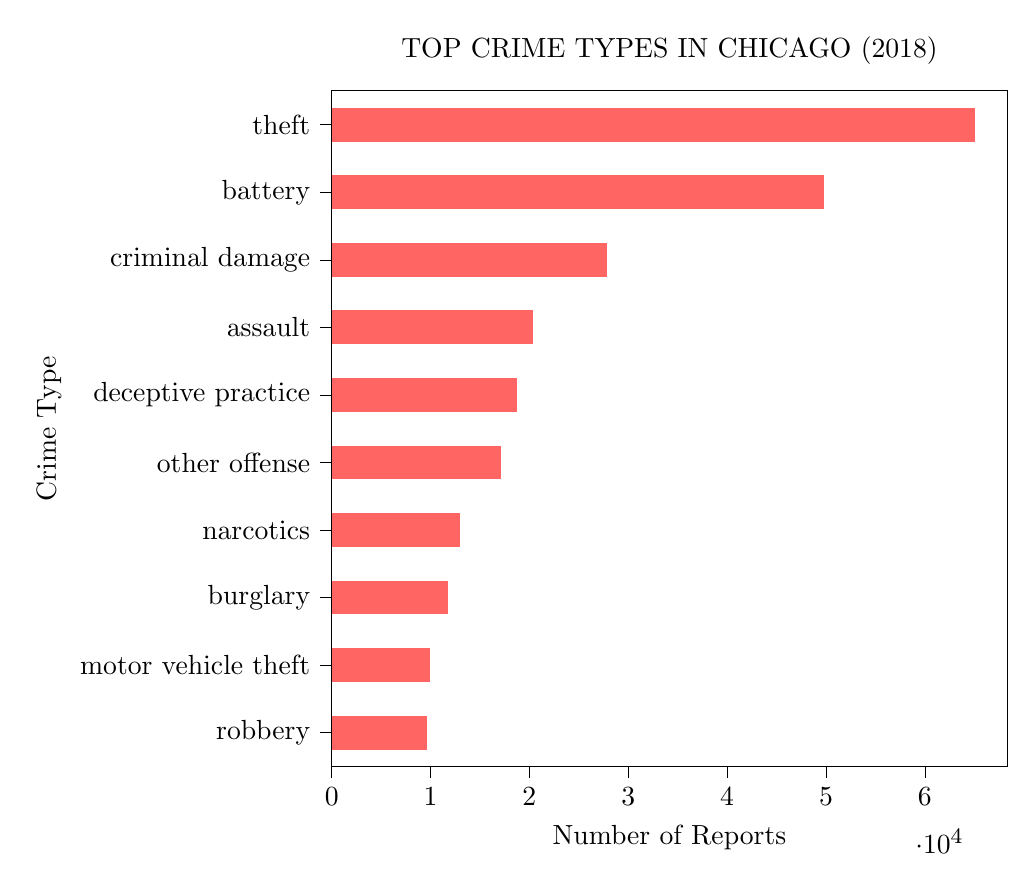
\begin{tikzpicture}

\definecolor{color0}{rgb}{1,0.4,0.388235294117647}

\begin{axis}[
height=4in,
tick align=outside,
tick pos=left,
title={\printsection{\MakeUppercase{Top Crime Types in Chicago (2018)}}},
width=4in,
x grid style={white!69.01960784313725!black},
xlabel={Number of Reports},
xmin=0, xmax=68332.95,
xtick style={color=black},
y grid style={white!69.01960784313725!black},
ylabel={Crime Type},
ymin=-0.5, ymax=9.5,
ytick style={color=black},
ytick={0,1,2,3,4,5,6,7,8,9},
yticklabels={robbery,motor vehicle theft,burglary,narcotics,other offense,deceptive practice,assault,criminal damage,battery,theft}
]
\draw[fill=color0,draw opacity=0] (axis cs:0,-0.25) rectangle (axis cs:9683,0.25);
\draw[fill=color0,draw opacity=0] (axis cs:0,0.75) rectangle (axis cs:9987,1.25);
\draw[fill=color0,draw opacity=0] (axis cs:0,1.75) rectangle (axis cs:11729,2.25);
\draw[fill=color0,draw opacity=0] (axis cs:0,2.75) rectangle (axis cs:12987,3.25);
\draw[fill=color0,draw opacity=0] (axis cs:0,3.75) rectangle (axis cs:17125,4.25);
\draw[fill=color0,draw opacity=0] (axis cs:0,4.75) rectangle (axis cs:18716,5.25);
\draw[fill=color0,draw opacity=0] (axis cs:0,5.75) rectangle (axis cs:20377,6.25);
\draw[fill=color0,draw opacity=0] (axis cs:0,6.75) rectangle (axis cs:27806,7.25);
\draw[fill=color0,draw opacity=0] (axis cs:0,7.75) rectangle (axis cs:49781,8.25);
\draw[fill=color0,draw opacity=0] (axis cs:0,8.75) rectangle (axis cs:65079,9.25);
\end{axis}

\end{tikzpicture}
\par}
\section{Data Augmentation \& APIs}
\subsection{Chicago Crime Reports, Augmented with ACS Demographic Information}
To pull in data from the American Community Survey, we need to identify which census tract each crime report corresponds to. This correspondence can be found by performing a \textit{spatial join}: with shapefiles representing the geometry of each Chicago-area census tracts as a polygon, each crime report's latitude/longitude pair can be assigned to a census tract based on which geometry contains the report's coordinates. Census tract shapefiles are available from the City of Chicago's Data Portal.
\begin{lstlisting}[language=Python,numbers=none]
from shapely.geometry import Point
import geopandas as gpd

def assign_census_tracts(crime_stats):
    boundary_shp = "./Boundaries - Census Blocks - 2000/geo_export_8e9f6d85-3c5b-429f-b625-25afcc3dea85.shp"
    census_tracts = gpd.read_file(boundary_shp).drop(columns=["perimeter", "shape_area", "shape_len"])
    # restrict geocoding to valid locations
    crime_stats = crime_stats[crime_stats["Location"].notna()]
    crime_stats["geometry"] = crime_stats.apply(lambda row: Point(row["Longitude"], row["Latitude"]), axis = 1)
    return gpd.tools.sjoin(gpd.GeoDataFrame(crime_stats), census_tracts, how="inner")
\end{lstlisting}

With the census tracts assigned, we can query the Census Bureau's API via DataMade's \texttt{census} Python package to find representative data about each census tract. We'll need the following ACS variables to pull in demographic data:

\begin{table}[H]
\centering \renewcommand{\arraystretch}{1.2}
\begin{tabular}{c|c}
\opns{ACS VARIABLE NAME} & \opns{LABEL} \\\hline 
\texttt{B01003\_001E} & total population \\
\texttt{B02001\_003E} & race (Black or African American alone) \\
\texttt{B03003\_001E} & Hispanic or Latino origin \\
\texttt{B19013\_001E} & median household income in the past 12 months \\
\texttt{B22002\_001E} & receipt of food stamps/SNAP in the past 12 months by children under 18 
\end{tabular}
\end{table}

\begin{lstlisting}[language=Python,numbers=none]
from census import Census

census_client = Census(census_api_key)

illinois = "17"
cook_county = "031"
acs_vars = {
    "NAME" : "tract_name",
    "B01003_001E": "total_pop",
    "B02001_003E": "black_pop",
    "B03003_003E": "hispanic_pop",
    "B19013_001E": "median_income",
    "B22002_001E": "child_snap"
}

tract_numbers = set(crime_stats["census_tra"].to_list())


response = census_client.acs5.state_county_tract(list(acs_vars.keys()), illinois, cook_county, Census.ALL)
demography = pd.DataFrame([elem for elem in response if elem["tract"] in tract_numbers]).rename(columns=acs_vars)
# normalize by population
demography[["black_pct", "hispanic_pct", "child_snap_pct"]] = demography[["black_pop", "hispanic_pop", "child_snap"]].div(demography.total_pop, axis=0)
demography["tract"] = pd.to_numeric(demography["tract"])
demography.set_index("tract")
crime_stats["census_tra"] = pd.to_numeric(crime_stats["census_tra"])
crime_stats = crime_stats.merge(demography, left_on=["census_tra"], right_on=["tract"])

demographic_vars = ["black_pct", "hispanic_pct", "child_snap_pct", "median_income"]

# battery
crime_stats[crime_stats["Primary Type"] == "BATTERY"][demographic_vars].describe()
# homicide
crime_stats[crime_stats["Primary Type"] == "HOMICIDE"][demographic_vars].describe()

# homicide over time 
crime_stats[(crime_stats["Primary Type"] == "HOMICIDE") & (crime_stats["Year"] == 2017)][demographic_vars].describe()
crime_stats[(crime_stats["Primary Type"] == "HOMICIDE") & (crime_stats["Year"] == 2018)][demographic_vars].describe()

# deceptive practice vs. sex offense 
crime_stats[crime_stats["Primary Type"] == "DECEPTIVE PRACTICE"][demographic_vars].describe()
crime_stats[crime_stats["Primary Type"] == "SEX OFFENSE"][demographic_vars].describe()

\end{lstlisting}

\subsubsection{What types of blocks have reports of “Battery”?}
\begin{table}[H]
\centering\renewcommand{\arraystretch}{1.2}
\begin{tabular}{lrrrr}
   &     \opns{\% BLACK} &  \opns{\% HISPANIC} &  \opns{\% CHILDREN ON SNAP} &  \opns{MEDIAN INCOME} \\\hline
   &      0.590492 &      0.197004 &        0.373272 &   43079.587196 \\
\end{tabular}
\end{table}

The typical block with incidents of battery is generally roughly 60\% Black and 20\% Hispanic. On average, 37\% of children receive food stamps, and the median income is about \$43,000.

\subsubsection{What types of blocks get “Homicide”?}
\begin{table}[H]
\centering\renewcommand{\arraystretch}{1.2}
\begin{tabular}{lrrrr}
   &   \opns{\% BLACK} &  \opns{\% HISPANIC} &  \opns{\% CHILDREN ON SNAP} &  \opns{MEDIAN INCOME} \\\hline
   &    0.732555 &      0.172105 &        0.352350 &   35031.494636 \\
\end{tabular}
\end{table}

The typical block with incidents of battery is generally roughly 73\% Black and 17\% Hispanic. On average, 35\% of children receive food stamps, and the median income is about \$35,000.

\subsubsection{Does that change over time in the data you collected?}
2017 Homicide characteristics:
\begin{table}[H]
\centering\renewcommand{\arraystretch}{1.2}
\begin{tabular}{lrrrr}
   &   \opns{\% BLACK} &  \opns{\% HISPANIC} &  \opns{\% CHILDREN ON SNAP} &  \opns{MEDIAN INCOME} \\\hline
   &    0.728826 &      0.185749 &        0.353375 &   34954.426374 \\
\end{tabular}
\end{table}

2018 Homicide characteristics:
\begin{table}[H]
\centering\renewcommand{\arraystretch}{1.2}
\begin{tabular}{lrrrr}
   &   \opns{\% BLACK} &  \opns{\% HISPANIC} &  \opns{\% CHILDREN ON SNAP} &  \opns{MEDIAN INCOME} \\\hline
   &    0.736974 &      0.155940 &        0.351134 &    35122.81250 \\
\end{tabular}
\end{table}

Comparing the 2017 to 2018 statistics, the characterization of the typical block for homicide stays effectively the same.

\subsubsection{What is the difference in blocks that get “Deceptive Practice” vs “Sex Offense”?}
Deceptive Practice:
\begin{table}[H]
\centering\renewcommand{\arraystretch}{1.2}
\begin{tabular}{lrrrr}
   &     \opns{\% BLACK} &  \opns{\% HISPANIC} &  \opns{\% CHILDREN ON SNAP} &  \opns{MEDIAN INCOME} \\\hline
   &      0.359146 &      0.182752 &        0.425968 &   65201.237182 \\
\end{tabular}
\end{table}

Sex Offense:
\begin{table}[H]
\centering\renewcommand{\arraystretch}{1.2}
\begin{tabular}{lrrrr}
   &    \opns{\% BLACK} &  \opns{\% HISPANIC} &  \opns{\% CHILDREN ON SNAP} &  \opns{MEDIAN INCOME} \\\hline
   &     0.413284 &      0.255555 &        0.385575 &   52807.952566 \\
\end{tabular}
\end{table}
Comparing the block characteristics between the two crime types, blocks with deceptive practice reports tend to have a higher median income (though also a higher percentage of children receiving food assistance). They also tend to have fewer Black or Hispanic residents than blocks with sex offense reports.

\section{Analysis \& Communication}
\subsection{Changes in Crime, 2017-2018}
By aggregating over the year of each report, or by the primary type of each reported crime, we can develop an overview of how crime has changed overall, and of how rates of each type of crime are changing.

\begin{lstlisting}[language=Python,numbers=none]
def summarize_changes(crime_stats):
    # overall changes
    crime_stats.groupby("Year").size().to_frame().T
    (100 * crime_stats.groupby("Year").size().pct_change()).to_frame().T

    # changes per type
    100 * crime_stats.groupby(["Primary Type", "Year"]).size().unstack().T.pct_change().stack().sort_values(ascending=False)
\end{lstlisting}

First, let us look at overall changes in crime:
\begin{table}[H]
\centering \renewcommand{\arraystretch}{1.2}
\begin{tabular}{l|rr|r}
year &    \opns{2017} &    \opns{2018} & \opns{\% change}\\\hline
number of reports    &  268094 &  266246 & -0.68931\\
\end{tabular}
\end{table}

The percentage change in overall crime is negligible; the total crime rate is effectively stable across 2017-2018.

\pagebreak 
Additionally, we can look at how each type of crime changed:

\begin{table}[H]
\centering \renewcommand{\arraystretch}{1.2}
\begin{tabular}{l|r}
  \opns{Primary Type}   &       \opns{\% Change, 2017-2018}  \\\hline
concealed carry license violation &  115.942029 \\
human trafficking &   55.555556 \\
non-criminal (subject specified) &   50.000000 \\
public indecency &   40.000000 \\
liquor law violation &   39.790576 \\
interference with public officer &   20.165746 \\
weapons violation &   16.303884 \\
narcotics &   11.399897 \\
intimidation &   11.258278 \\
stalking &    7.978723 \\
sex offense &    7.609756 \\
assault &    5.563902 \\
gambling &    5.235602 \\
criminal trespass &    1.350558 \\
battery &    1.152111 \\
theft &    1.140726 \\
crim sexual assault &   -0.061425 \\
other offense &   -0.592094 \\
obscenity &   -1.149425 \\
deceptive practice &   -1.624179 \\
offense involving children &   -1.718819 \\
prostitution &   -2.312925 \\
non-criminal &   -2.631579 \\
criminal damage &   -4.255905 \\
public peace violation &   -8.611482 \\
burglary &   -9.783863 \\
kidnapping &  -11.052632 \\
motor vehicle theft &  -12.440821 \\
homicide &  -13.313609 \\
arson &  -16.216216 \\
robbery &  -18.472678 \\
other narcotic violation &  -90.909091 \\
\end{tabular}
\end{table}
Clearly, not all types of crimes are changing at the same rates. Concealed carry license violations more than doubled between 2017 and 2018, while other narcotic violations dropped by 90\%.
\pagebreak
\subsection{Analysis of Jacob Ringer's Claims}
Jacob Ringer, a candidate for alderman for the 43rd Ward, claims: 

\begin{mdframed}[topline=false, bottomline=false, rightline=false,linewidth=2pt,linecolor=gray]
Let's break down the Chicago Police Department's report for the month leading up to July 26, 2018, compared to the same week [\textit{sic}] in 2017:
\begin{itemize}
\item Robberies -- up 21 percent over the same time-frame in 2017
\item Aggravated batteries -- up 136 percent
\item Burglaries -- an increase of 50 percent
\item Motor vehicle theft -- up 41 percent.
\end{itemize}
All told, crime rose 16 percent in the same 28-day time period in just one year.
\end{mdframed}

To evaluate Ringer's claims, we can filter down the relevant ward, and isolate the time periods he analyzes.
\begin{lstlisting}[language=Python,numbers=none]
import datetime

one_month = datetime.timedelta(days = 28) # "same 28-day time period in just one year"
target17 = datetime.datetime(year=2017, month=7, day=26)
target18 = datetime.datetime(year=2018, month=7, day=26)

crime_stats = crime_stats[crime_stats["Ward"] == 43]
crime_stats["Date"] = pd.to_datetime(ward_crime_stats["Date"])
crime_stats = crime_stats[
    ((target17 - one_month <= crime_stats["Date"]) & (crime_stats["Date"] <= target17)) | 
    ((target18 - one_month <= crime_stats["Date"]) & (crime_stats["Date"] <= target18))
]

# overall changes
crime_stats.groupby("Year").count()["ID"]
crime_stats.groupby("Year").count()["ID"].pct_change()

crime_stats = crime_stats[crime_stats["Primary Type"].isin(["ROBBERY", "BATTERY", "BURGLARY", "MOTOR VEHICLE THEFT"])]
crime_agg_2017 = crime_stats[crime_stats["Year"] == 2017]["Primary Type"].value_counts()
crime_agg_2018 = crime_stats[crime_stats["Year"] == 2018]["Primary Type"].value_counts()
crime_agg_2017.name, crime_agg_2018.name = "2017", "2018"
pd.DataFrame([crime_agg_2017, crime_agg_2018])
\end{lstlisting}

Calculated changes in crime for the 43rd ward:
\begin{table}[H]
\centering \renewcommand{\arraystretch}{1.2}
\begin{tabular}{l|rr|rr}
\multicolumn{1}{l|}{} & & & \opns{ACTUAL} & \opns{CLAIMED} \\
\multicolumn{1}{l|}{year} &    \opns{2017} &    \opns{2018} &     \opns{\% CHANGE} &     \opns{\% CHANGE} \\\hline
\multicolumn{1}{l|}{all crimes}          &  340  &  378   &  +11.18 \% & +16  \% \\
\multicolumn{1}{l|}{battery}             &    38 &    33  & -13.16  \% & +136 \% \\
\multicolumn{1}{l|}{robbery}             &    17 &     8  & -52.94  \% & +21  \% \\
\multicolumn{1}{l|}{burglary}            &    16 &    13  & -18.75  \% & +50  \% \\
\multicolumn{1}{l|}{motor vehicle theft} &     5 &    10  & +100.00 \% & +41  \% \\
\end{tabular}
\end{table}
\pagebreak
Further, Ringer claims:
\begin{mdframed}[topline=false, bottomline=false, rightline=false,linewidth=2pt,linecolor=gray]
But take a look at the year-to-date number and you'll see how crime has affected our local neighborhoods in a four-year period:
\begin{itemize}
\item Rose 10 percent since 2017
\item Rose 22 percent since 2016
\end{itemize}
\end{mdframed}
Since we have data for 2017 and 2018, we can analyze the first claim in this section: 
\begin{lstlisting}[language=Python,numbers=none]
def analyze_ward_to_date(crime_stats, ward=43, target_month=7, target_day=26):
    year_start = lambda year: datetime.datetime(year=year, month=1, day=1)
    to_date = lambda year: datetime.datetime(year=year, month=target_month, day=target_day)
    crime_stats = crime_stats[crime_stats["Ward"] == ward]
    crime_stats["Date"] = pd.to_datetime(crime_stats["Date"])
    crime_stats = crime_stats[
        ((year_start(2017) <= crime_stats["Date"]) & (crime_stats["Date"] <= to_date(2017))) | 
        ((year_start(2018) <= crime_stats["Date"]) & (crime_stats["Date"] <= to_date(2018)))
    ]

    crime_stats.groupby("Year").size()
    crime_stats.groupby("Year").size().pct_change()
analyze_ward_to_date(crime_stats, ward=43, target_month=7, target_day=26)
analyze_ward_to_date(crime_stats, ward=43, target_month=12, target_day=31)
\end{lstlisting}

\begin{table}[H]
\centering \renewcommand{\arraystretch}{1.2}
\begin{tabular}{l|rr|rr}
{}   & {}             &                & \opns{ACTUAL} & \opns{CLAIMED} \\
year &    \opns{2017} &    \opns{2018} & \opns{\% change} & \opns{\% change} \\\hline
year-to-date number of reports in ward 43   &  2148 &  2359 & +9.823\% & +10\%\\
\end{tabular}
\end{table}

Ringer's claim about the comparison of crime reports from the start of the year to 26 July of each year is correct. However, there is no reason why 26 July is a useful cut-off in analyzing crime rates. Looking at crime reports in ward 43 for \textit{the whole year} indicates crime reports rose by 7.55\%.
In general, while some of Ringer's claims are directionally correct, his crime statistics should be rejected overall, and we cannot trust any conclusions made from these statistics.
\subsection{Key Findings}
\begin{enumerate}
\item The total amount of crime in Chicago is effectively constant across the time period 2017-2018.
\item The majority of crime across the time period analyzed is dominated by incidents of: theft, battery, criminal damage, and assault. 
\item The proportion of motor vehicle theft and narcotics crimes are growing from 2017 to 2018, while robbery incidents are proportionally decreasing.
\item The fastest-growing (specific) types of crime are: concealed carry license violation, human trafficking, public indecency and liquor law violations. Crime prevention efforts should focus on these categories.
\item Crime types whose prevalence is falling include: homicide, arson, robbery, and other narcotic violation.
\end{enumerate}
\subsection{Caveats \& Limitations}
Some caveats apply to this analysis:
\begin{itemize}
\item Demographic information comes from the American Community Survey, in which responses are voluntary. These data may therefore be incomplete or flawed due to non-response.
\item Statistics solely about crime are from a two-year window; a more comprehensive analysis would take into account several years of crime statistics.
\end{itemize}

\section{Probability Exercise}
\subsection{Probabilities of Crime Type for a Call from a Given Address}
We can aggregate the crime types for the given block to see that battery is the most probably report type for the block at 2111 S Michigan Ave. The overall probabilities can also be calculated: 

\begin{lstlisting}[language=Python, numbers=none]
def analyze_crime_for_block(crime_stats, block_address):
    return 100 * crime_stats[crime_stats["Block"].str.contains(block_address)]["Primary Type"].value_counts(normalize=True)

analyze_crime_for_block(crime_stats, "021XX S MICHIGAN")
\end{lstlisting}
\begin{table}[H]
\centering \renewcommand{\arraystretch}{1.2}
\begin{tabular}{l|r}
\opns{Primary Type} &  \opns{Probability} \\\hline
battery                &     26.667\% \\
other offense          &     21.667\% \\
criminal damage        &     10.000\% \\
theft                  &     10.000\% \\
assault                &     10.000\% \\
deceptive practice     &     10.000\% \\
robbery                &      3.333\% \\
motor vehicle theft    &      3.333\% \\
burglary               &      1.667\% \\
public peace violation &      1.667\% \\
criminal trespass      &      1.667\% \\
\end{tabular}
\end{table}

\subsection{Theft in Garfield Park vs. Uptown}
The City of Chicago's Data Portal indicated that Garfield Park corresponds to community areas 26 and 27 and Uptown to community area 3. With this mapping, we can aggregate community areas over reports of theft and find the probabilities:

\begin{lstlisting}[language=Python,numbers=none]
def theft_probabilities(crime_stats, areas):
    return 100 * crime_stats[crime_stats["Primary Type"] == "THEFT"]["Community Area"].value_counts(normalize=True)[[float(a) for a in areas]]

theft_probabilities(crime_stats, [26, 27, 3])  
\end{lstlisting}

\begin{table}[H]
\centering \renewcommand{\arraystretch}{1.2}
\begin{tabular}{r|r}
\opns{Community}      & \opns{Probability of Origin,} \\
\opns{Area} &  \opns{given theft call} \\\hline
26.0 &        0.937\% \\
27.0 &        0.990\% \\
3.0  &        1.510\% \\
\end{tabular}
\end{table}

The total probability of the call being from Garfield Park is 1.927\%, which is 0.42 percentage points more likely than Uptown.

\subsection{Calculation under Simulated Frequencies}
We can use Bayes' Theorem to calculate the conditional probabilities:

$$ P\left( A\middle\vert B\right) = \frac{P\left( B\middle\vert A\right) P\left( A\right) }{P\left( A\right)} $$

From the problem statement, we know: 
\begin{multicols}{2}
$$ P\left(\opns{GARFIELD PARK}\right) = \frac{600}{1000}  = 0.6 $$

$$ P\left(\opns{UPTOWN}\right) = \frac{400}{1000}  = 0.4 $$

$$ P\left(\opns{BATTERY}\right) = \frac{100 + 160}{1000}  = 0.26 $$

$$ P\left(\opns{BATTERY} \middle\vert \opns{GARFIELD PARK} \right) = \frac{100}{600}  = 0.16667 $$

$$ P\left(\opns{BATTERY} \middle\vert \opns{UPTOWN} \right) = \frac{160}{400}  = 0.4 $$
\end{multicols}

Therefore, 

$$ P\left(\opns{GARFIELD PARK} \middle\vert \opns{BATTERY} \right) = \frac{P\left( \opns{BATTERY} \middle\vert \opns{GARFIELD PARK}\right) P\left( \opns{GARFIELD PARK}\right) }{P\left(\opns{BATTERY}\right)}$$
$$ = \frac{0.16667\cdot 0.6}{0.26} = 0.3846 $$

$$ P\left(\opns{UPTOWN} \middle\vert \opns{BATTERY} \right) = \frac{P\left( \opns{BATTERY} \middle\vert \opns{UPTOWN}\right) P\left( \opns{UPTOWN}\right) }{P\left(\opns{BATTERY}\right)}$$
$$ = \frac{0.4\cdot 0.4}{0.26} = 0.6154 $$

From these calculations, a call about battery is 23\% more likely to come from Uptown than from Garfield Park.
\pagebreak
\section*{Sources}
\begin{itemize}

\item "Boundaries - Census Blocks - 2000." City of Chicago | Data Portal. Accessed April 10, 2019. \url{https://data.cityofchicago.org/Facilities-Geographic-Boundaries/Boundaries-Census-Blocks-2000/uktd-fzhd}.

\item "Boundaries - Census Tracts." City of Chicago. Accessed April 10, 2019. \url{https://www.chicago.gov/city/en/depts/doit/dataset/boundaries_-_censustracts.html}.

\item "Boundaries - Census Tracts." Boundaries - Census Tracts. Accessed April 10, 2019. \url{https://www.chicago.gov/city/en/depts/doit/dataset/boundaries_-_censustracts.html}.

\item  McKinney, Wes. \textit{Python for Data Analysis: Data Wrangling with Pandas, NumPy, and IPython}. First Beijing: O'Reilly, 2013. 

\item Ringer, Jacob. "Crime in the 43rd Ward." Ringer4Results. Accessed April 10, 2019.\url{https://www.ringer4results.com/node/8}.

\item "Datamade/census." GitHub. February 09, 2019. Accessed April 10, 2019. \url{https://github.com/datamade/census}.

\item "Merging Data." Merging Data - GeoPandas 0.4.0 Documentation. Accessed April 10, 2019. \url{http://geopandas.org/mergingdata.html}.
\end{itemize}

\end{document} 
